\graphicspath{{intro/images}}

\newcommand{\maxwidth}{\textwidth}
\newcommand{\maxheight}{0.44\textheight}
\newcommand{\maxlessheight}{0.35\textheight}

\section{Начало работы в WokWi}

\subsection{Создание проекта}

\begin{enumerate}

    \item Вид главной страницы Wokwi:
    
    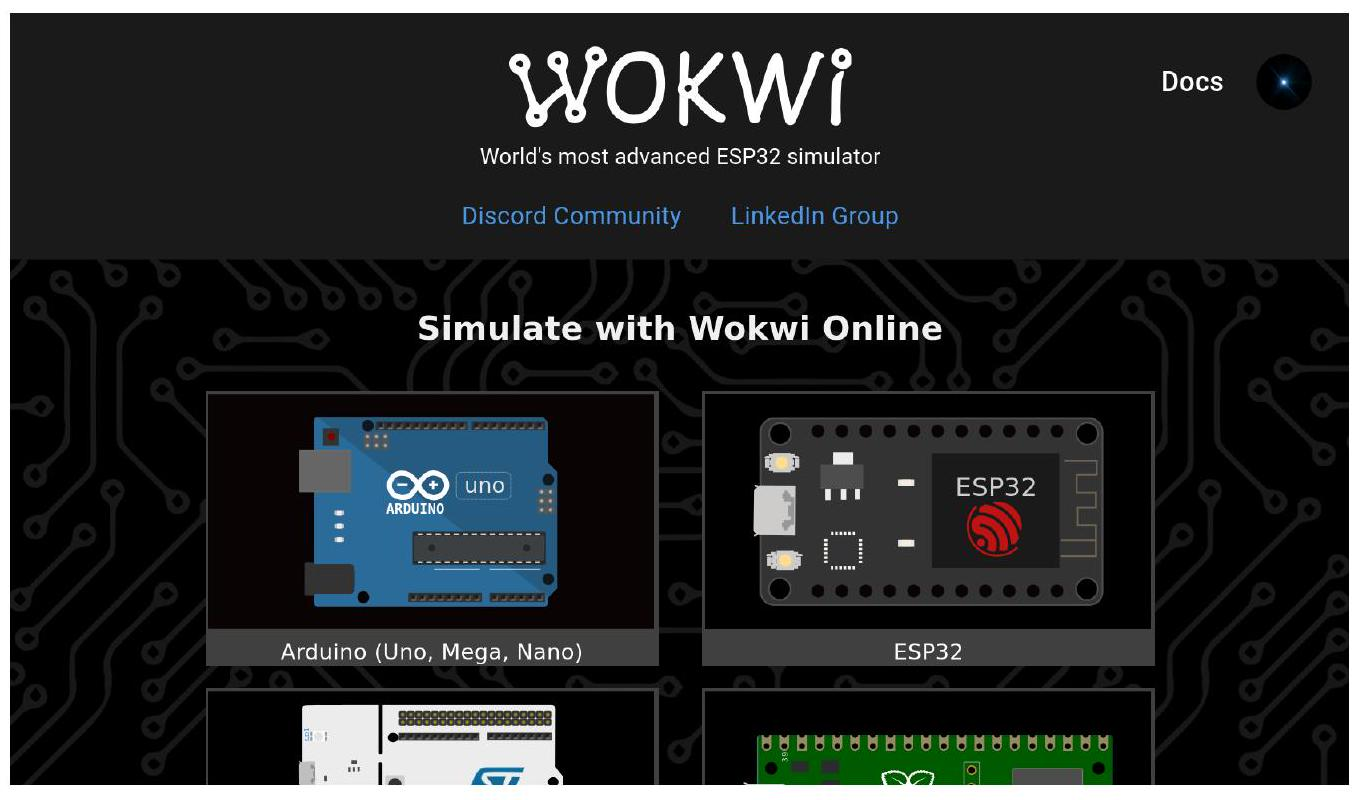
\includegraphics[max width=\maxwidth, max height=\maxlessheight, center]{1.jpg}    
    
    \item Откройте выпадающее меню профиля и нажмите кнопку "Мои проекты"\\
    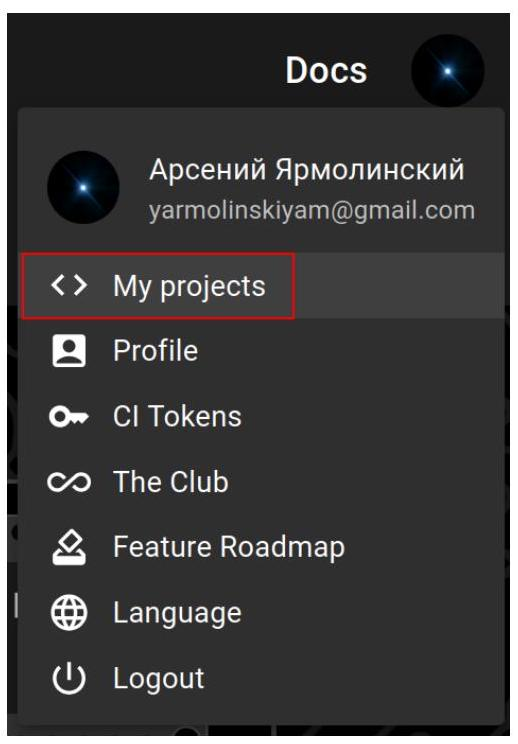
\includegraphics[max width=\maxwidth, max height=\maxheight, center]{2}
    
    \clearpage\item Страница проектов\\
    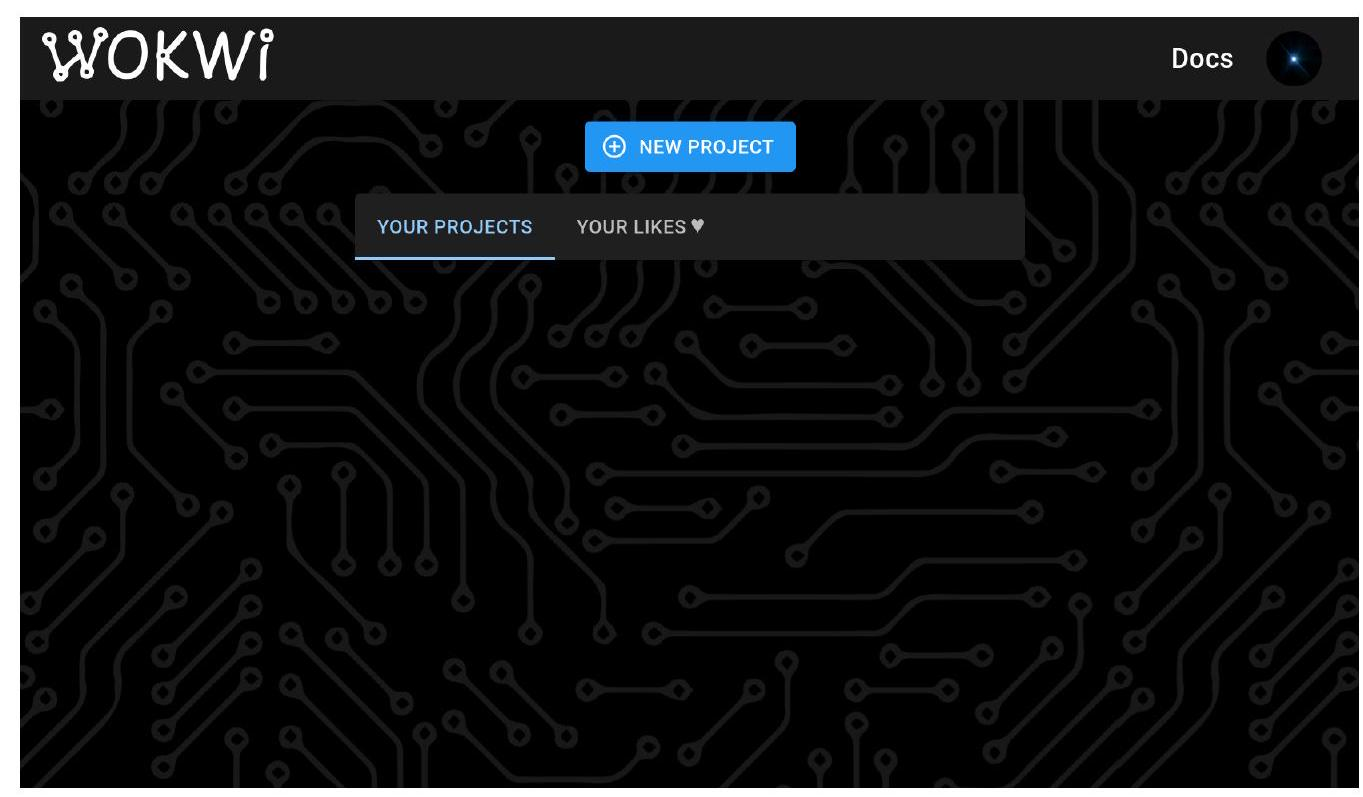
\includegraphics[max width=\maxwidth, max height=\maxheight, center]{3}
    
    \item Создайте новый проект\\
    
\includegraphics[max width=\maxwidth, max height=\maxheight, center]{4}
    
    \clearpage\item Выберите в меню слева семейство контроллеров Arduino\\
    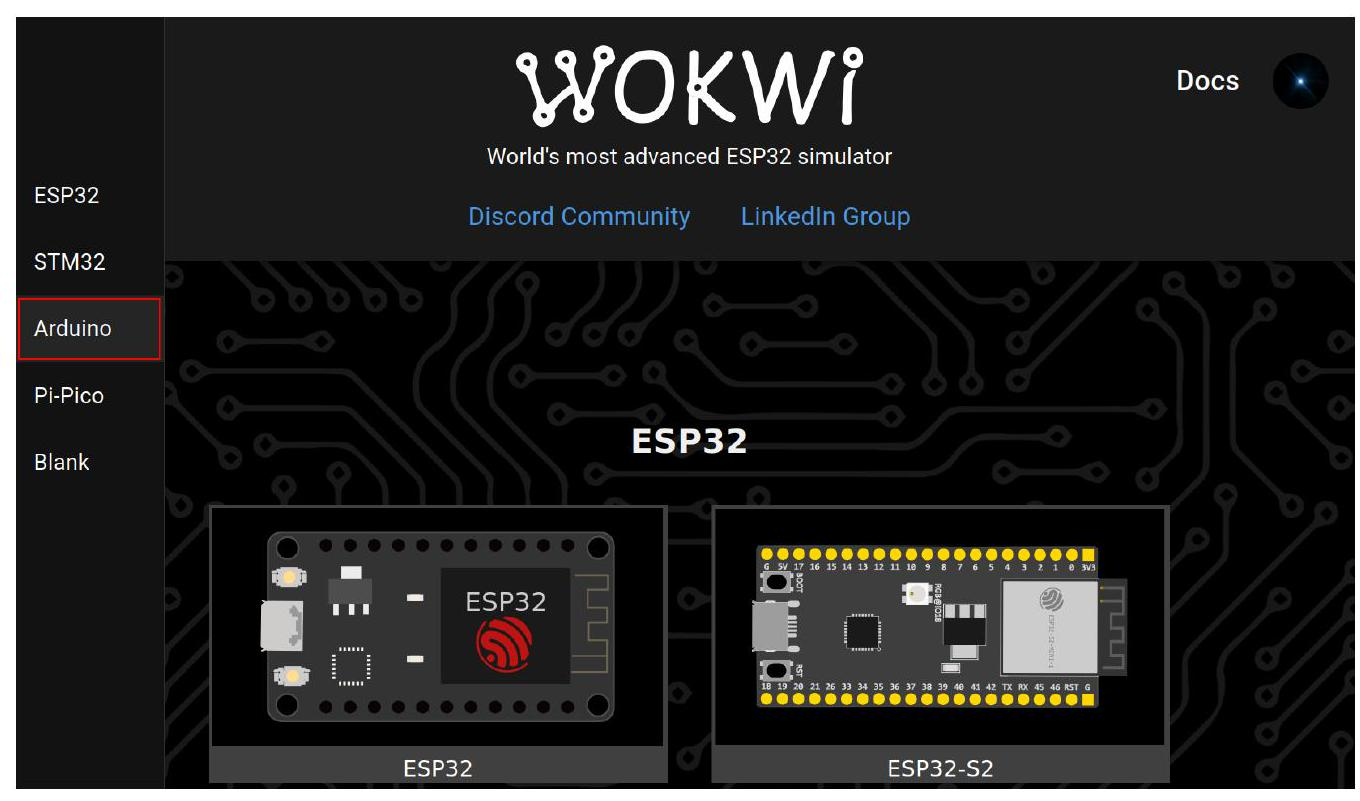
\includegraphics[max width=\maxwidth, max height=\maxheight, center]{5}
    
    \item Выберите контроллер Arduino Uno Rev3\\
    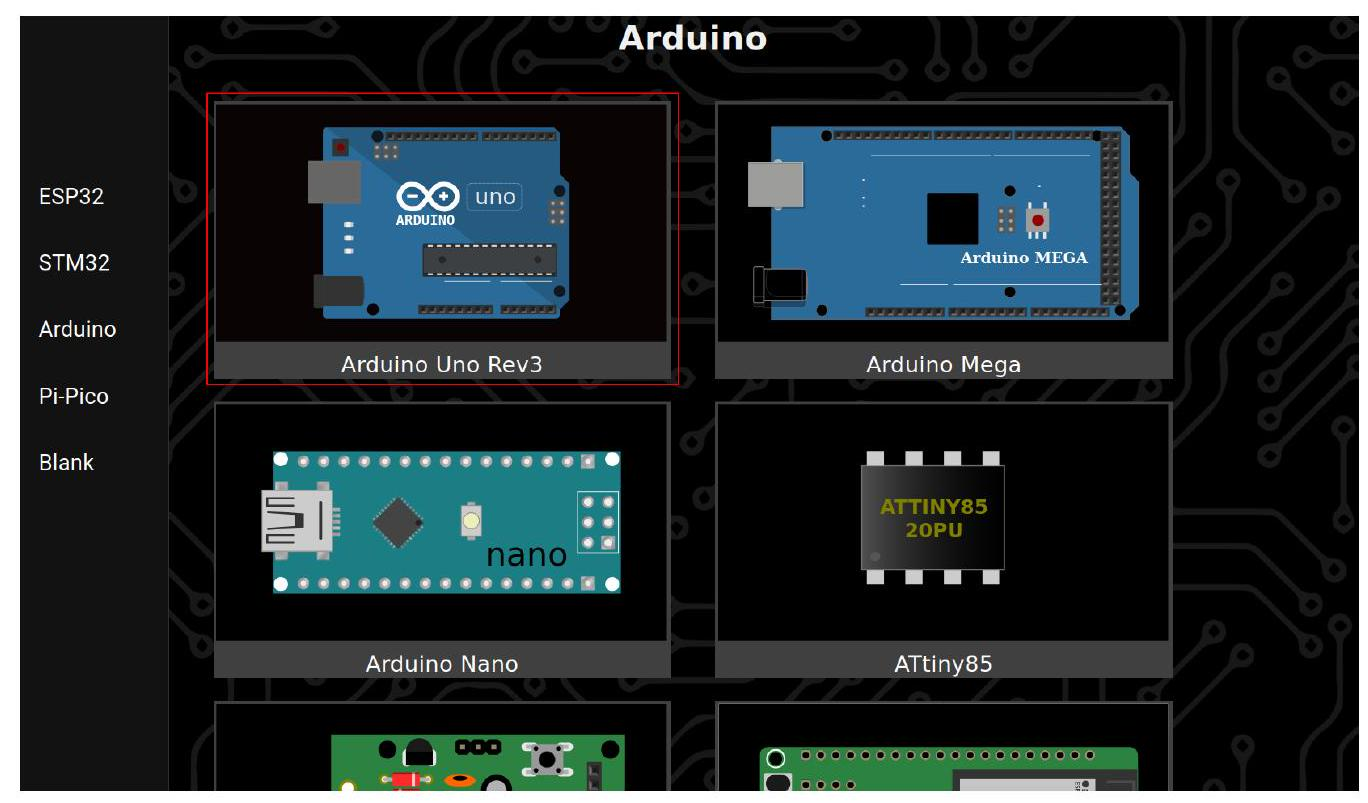
\includegraphics[max width=\maxwidth, max height=\maxheight, center]{6}

    \clearpage\item Созданный пустой проект!\\
    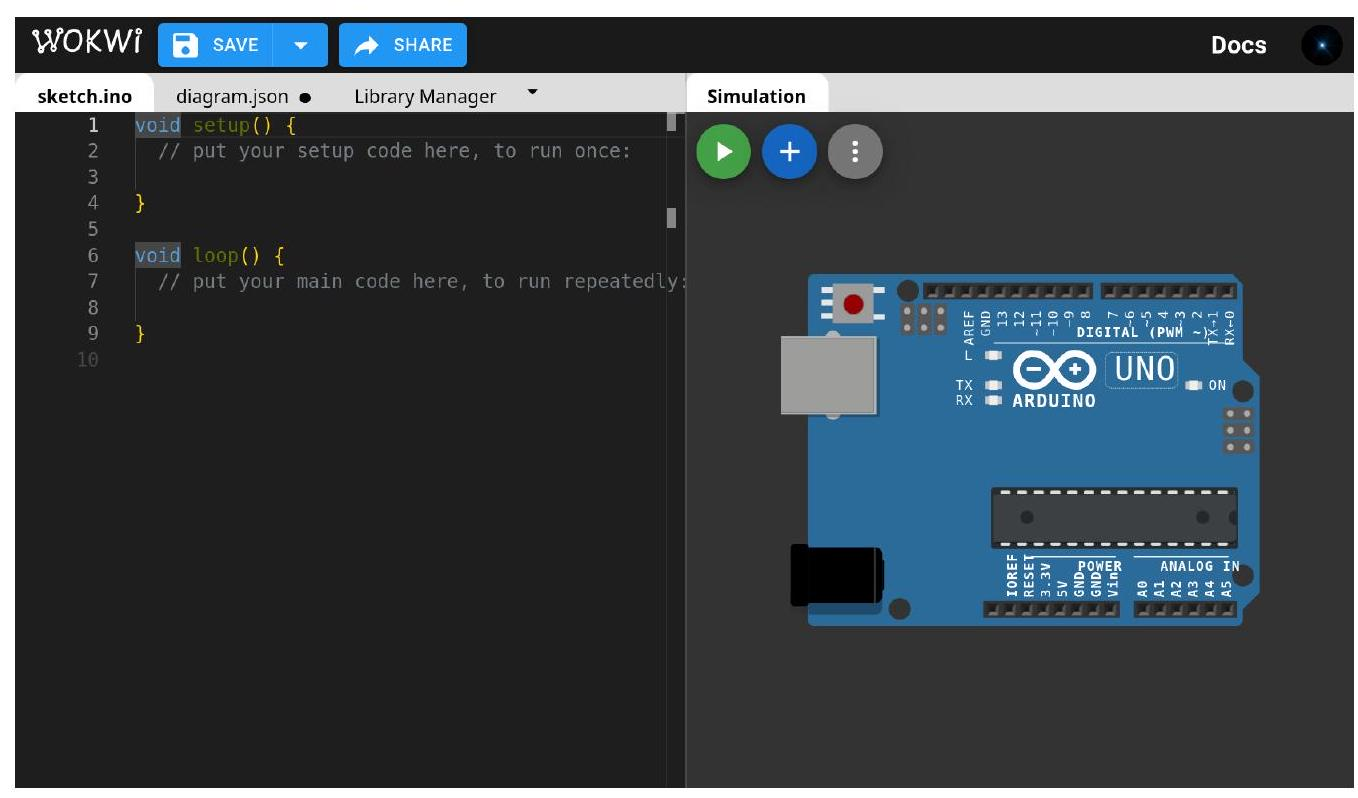
\includegraphics[max width=\maxwidth, max height=\maxheight, center]{7}

    \item После внесения изменений сохраните проект с помощью кнопки SAVE\\
    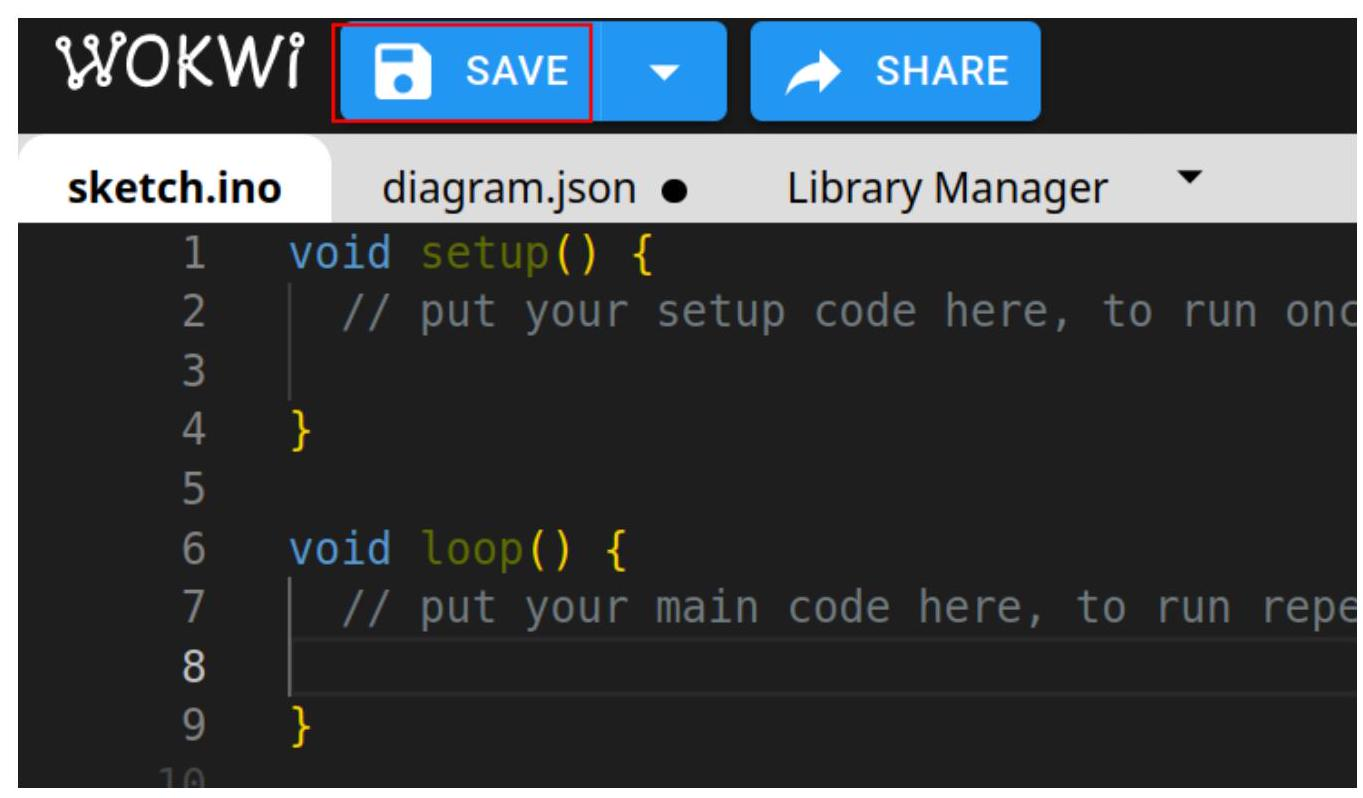
\includegraphics[max width=\maxwidth, max height=\maxheight, center]{8}

    \clearpage\item Введите название проекта и убедитесь, что он сохраняется как Public\\
    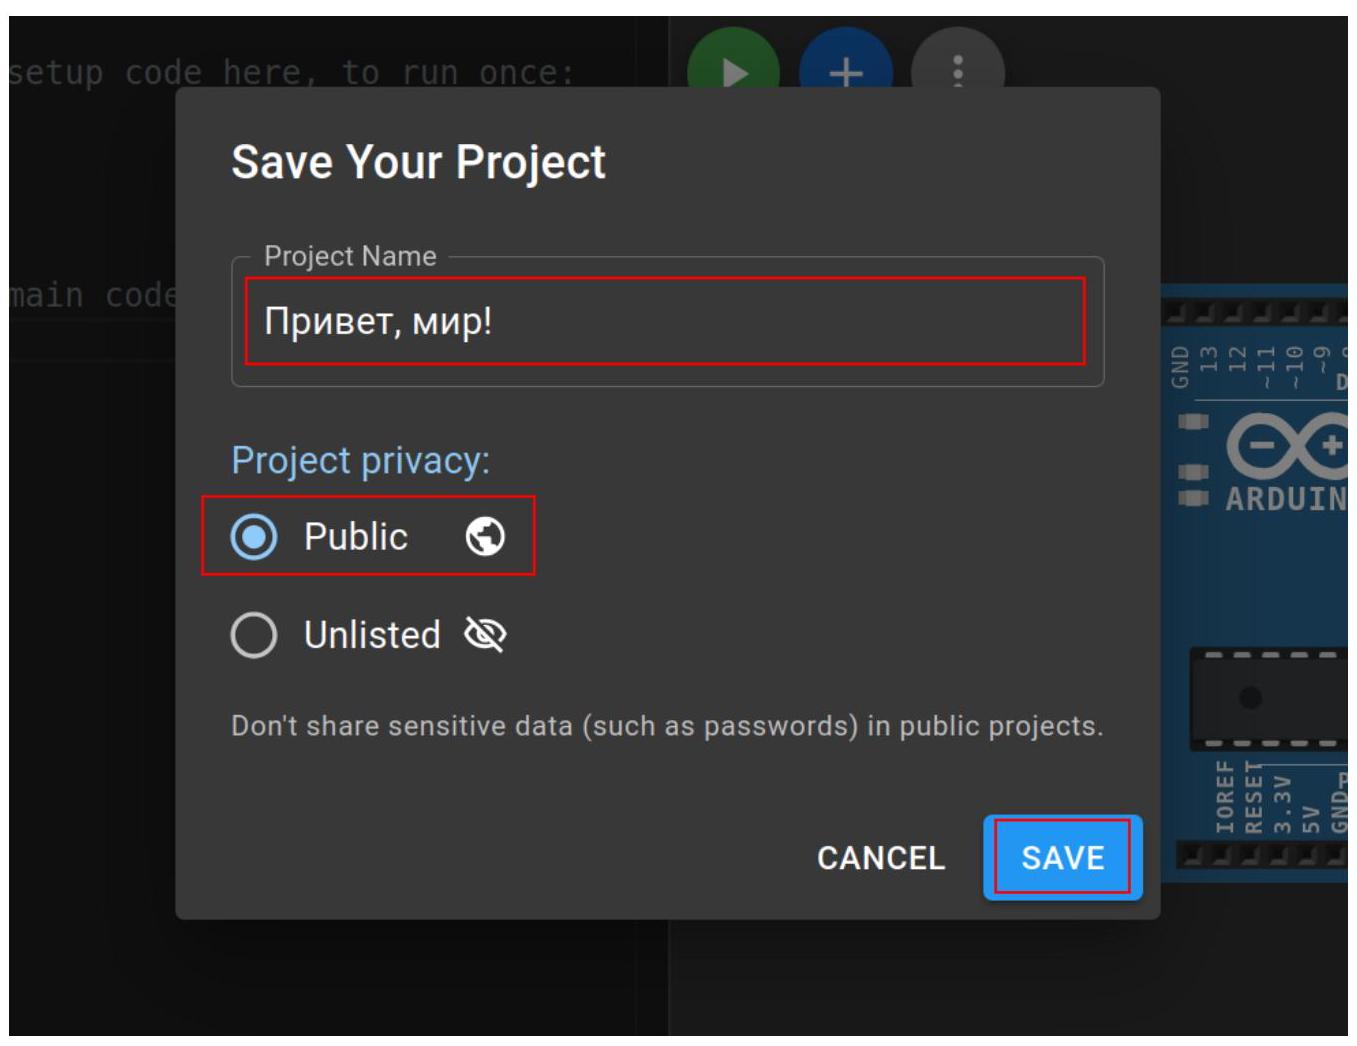
\includegraphics[max width=\maxwidth, max height=\maxheight, center]{9}

    \item Для добавления новой детали нажмите кнопку добавления\\
    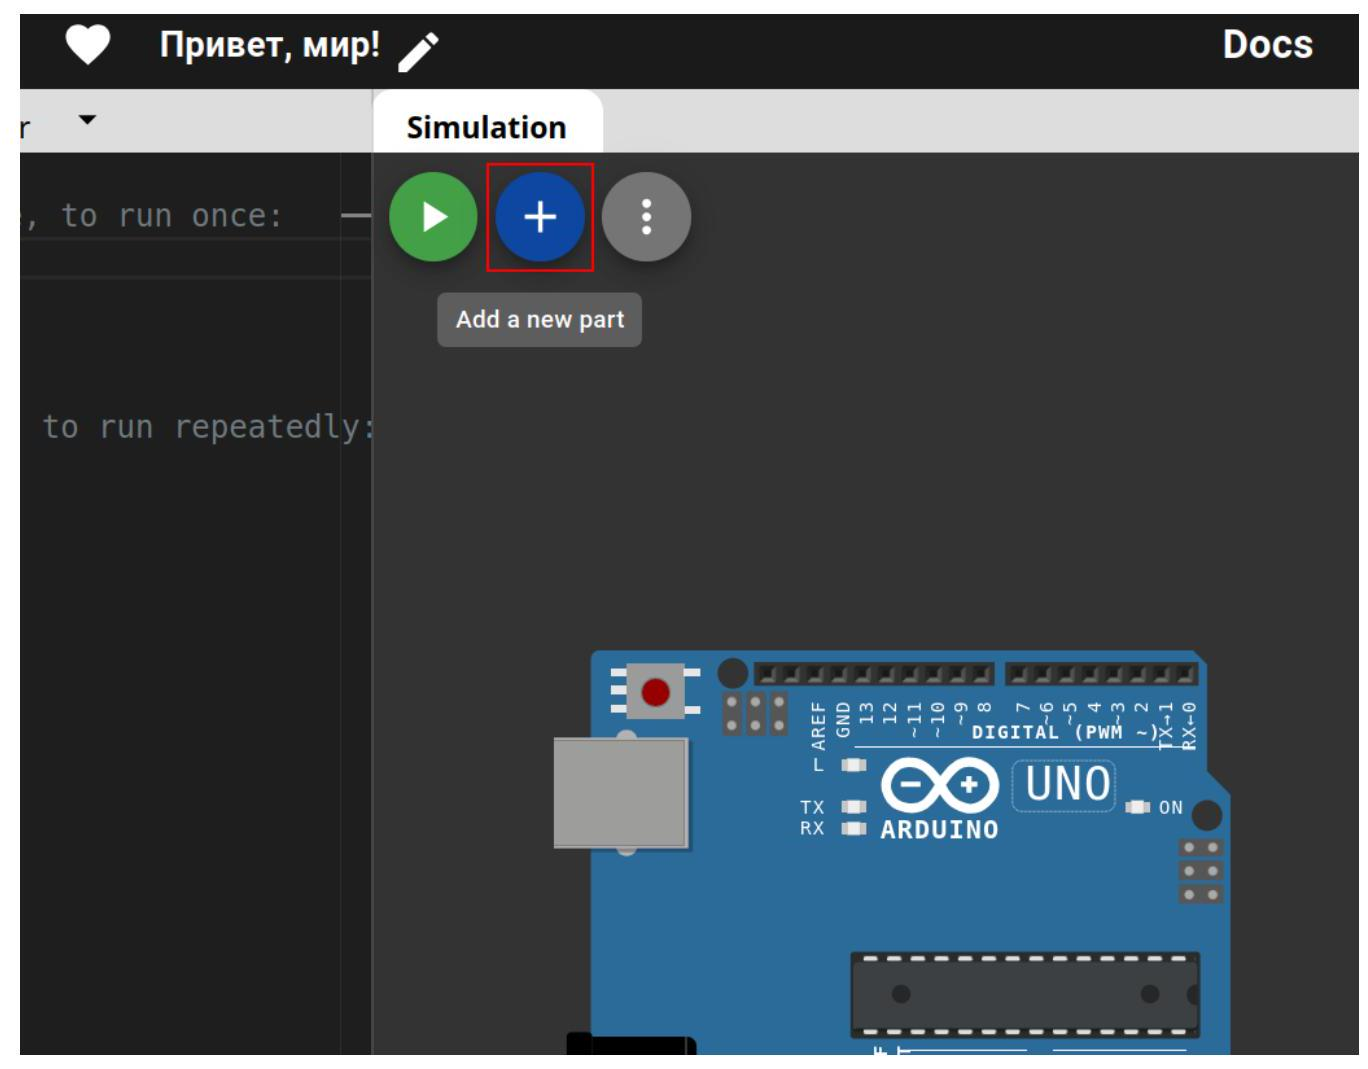
\includegraphics[max width=\maxwidth, max height=\maxheight, center]{10}

    \clearpage\item И выберите нужную деталь из выпадающего меню\\
    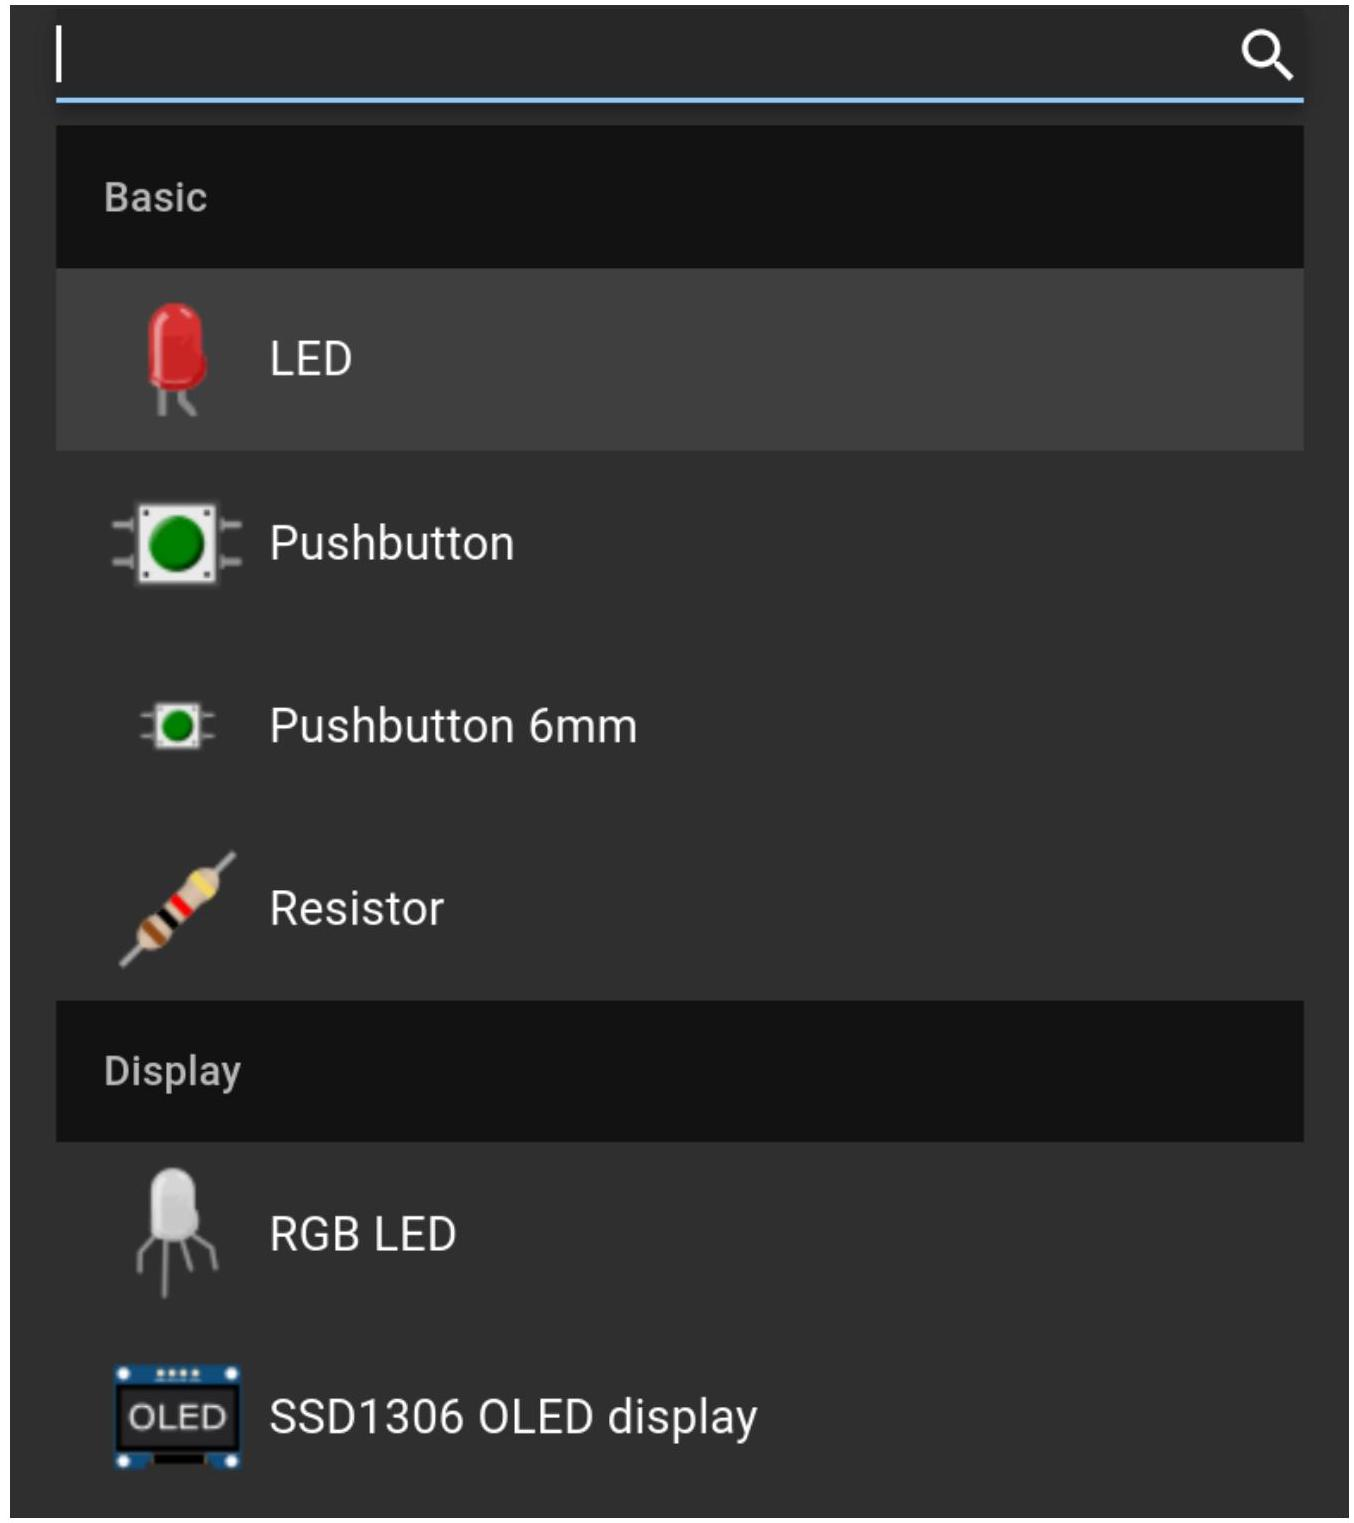
\includegraphics[max width=\maxwidth, max height=\maxheight, center]{11}

\end{enumerate}
% \begin{figure}[htbp]
%     \centering
%     \caption{<caption>}
%     \label{<label>}
% \end{figure}
